\chapter{Data Distribution Service}
\section{Overview}
The concept of distributed applications is to enable seamless communication between systems. There are a number of different ways to achieve this and the one we are focusing on is Data distribution service for real-time systems (DDS).
It is a standard developed by Object Management Group (OMG) that enables communication between computers, that is decoupled in space, time and flow. This means that the computers don't have to know each other and they don't have to be ready to receive when a message is sent. It uses a publish/subscribe pattern to send and receive messages that can be customised by a list of quality of service parameters.

\section{Middleware}

\subsection{What and why?}
To achieve this seamless communication some layer of software is needed to handle the network communication and distribution of data. This layer of software is called middleware.

Middleware can be defined by this quote:

"A layer of software residing on every machine, sitting between the
underlying operating system and the distributed applications,
whose purpose is to mask the heterogeneity of the cooperating
platforms and provide a simple, consistent and integrated
distributed programming environment."\footnote{\citep{DistributedSystems}}

DDS implements the Publish/Subscribe middleware paradigm that is described in the next section.

\subsection{Alternatives to DDS}

There are a number of different implementations of middleware in distributed systems where Publish/Subscribe as used in DDS is just one example. An alternative is Enterprise Messaging System (EMS) that is a set of standards that allows organisations to send messages between computer systems using standard formats like XML and SOAP.
TIBCO Enterprise Messaging Service is an example of implementation of EMS.

TIBCO EMS could be used as a real time messaging system in a big cooperation. It is secure as it uses TSL/SSL, it is reliable and scalable via load balancing and guaranteed message delivery models. And it supports a wide array of technologies that secures easy development and reuse of existing systems.

\section{Publish/Subscribe pattern}
The publish/subscribe pattern is a well known programming paradigm. It is more well known in the form of the Observer Pattern described by Gang of Four \footnote{\citep{DesignPatterns}}
The idea of the publish/subscribe pattern is loosening the coupling between a publisher and a subscriber. A publisher is a entity that has some data or content to deliver or distribute. A subscriber is interested in obtaining this information when it is published, but without needing to know where it is published from.
The subscriber subscribes to a topic or type at a EventService of some kind. When a publisher notifies the EventService with the new data, The EventService will notify the concerned subscribers. This is illustrated in the figure below.

\begin{center}
	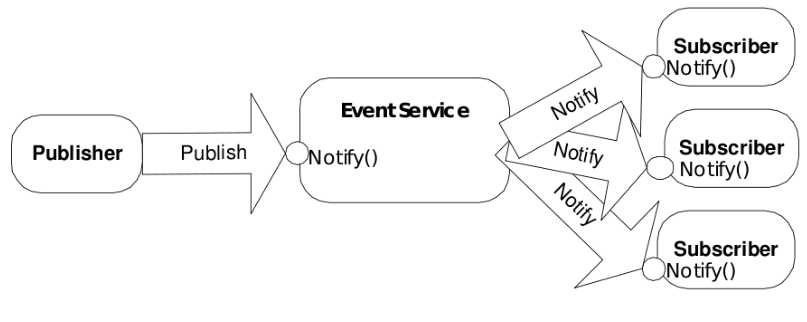
\includegraphics[width=\textwidth]{PublishSubscribe_Pattern.png}
	\captionof{figure}{Sublish/Subscribe pattern}
\end{center}

This is the same approach used by DDS. The Middleware must act as the EventService, and the application implements the publisher and subscriber.

\subsection{Data-Centric Publish-Subscribe}
Publishing and Subscribing in DDS is Data-centric, in that everything is bound to the type/topic/content of the DATA. Subscribers only get the data they need/want and get to filter based on contents, keys and types. 
The terms of the coupling between the Publishers and Subscribers are set up based on the data (see Quality of Service). The Data-Centric Publish-Subscribe interface is built directly from this model. Messages are being passed back and forth to the middleware and used by upper-layer applications.

\subsection{Data Local Reconstruction Layer}
An optional Data Local Reconstruction Layer (DLRL) can be added on top of the DCPS layer. This layer will give a further layer of abstraction from Application <--> Middleware. 
This layer will take sent data and automatically update certain fields in local classes, so that data, that is really located remotely, will appear local. This will also make it possible to make complicated remote method calls, as if they were local. 

\subsection{Interface Definition Language}
To be able to use features such as DLRL, remote endpoints and the local applications must have a common "language" to describe certain interfaces and classes. This common language is the Interface Definition Language (IDL).

Using this language as markup, two remote location can "talk" even though they are written in different programming languages!

IDL descriptions are needed, if one is to use the DLRL, as the DLRL entities are created from IDL. 

\subsection{Coupling}
There are tree types of coupling. Coupling in Space, Flow and Time.

\textbf{Space decoupling} is when the publisher and subscriber do not have to know each other. This is done by the introduction of the EventService.  Here the data is routed from the publisher through to every subscriber that needs this data. It is not necessary to pass references between the entities.

\textbf{Flow decoupling} is when the flow of the program will not be blocked. For example it is not necessary for the publisher to have a subscriber to deliver the message to, since it will be consumed (and maybe stored) by the EventService. 

\textbf{Time decoupling} is, when the time of delivery/reception of a message is independent on the time of transmission. As shown in the figure below, the subscriber will receive the published message, despite the fact that is has not been connected at the time of transmission AND the publisher has been disconnected since.

\begin{center}
	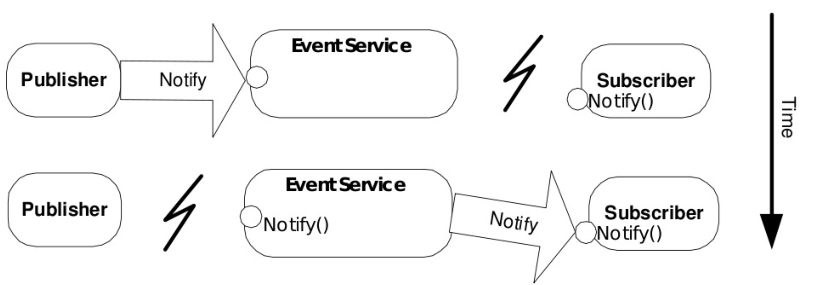
\includegraphics[width=\textwidth]{TimeDecoupling.png}
	\captionof{figure}{Illustration shwong decoupling in time from 02DDS Slideshow}
\end{center}

The Data Distribution Service as specified by OMG enables decoupling in all three  dimensions. This is defined through the use of Quality Of Service profiles.

\subsection{Filtering}
There are three different ways of publishing and subscribing to messages:

\textbf{Topic based} publishing is a way of distributing data based on the topic of it. The publisher is responsible of defining the topic of a message when it is dispatched. The subscriber has to subscribe to these exact topics.

\textbf{Content based} subscription is aimed at receiving data based on the content of it. The subscriber must utilize some filters which defines attributes or content that must be set.

\textbf{Type based} is subscription that is based on member types. This enables for implementation closer bound to the programming language.


\section{Real-time systems}
A real-time system is one that "controls an environment by receiving data, processing them, and returning the results sufficiently quickly to affect the environment at that time." \footnote{\citep{ProgrammingRealTimeComputerSystem}}

If the system can't deliver a response in the given time frame then there will typically be some kind of consequence.

\section{Quality Of Service}
For setting up the connections between entities, Publishers, Middleware and Subscribers must agree on certain terms. Quality of Service (QoS) lets the middleware know how to treat connections between publishers and subscribers as well as how to treat messages.

The QoS lets us setup \textit{terms} of the communication. This can be used, for instance, to set up the \textit{lifetime} of a message. This way, we could make sure a message will stop being interesting to subscribers after a while. 

Another example is setting the \textit{deadline} parameter on a subscribers QoS. This tells publishers, that the subscriber expects data within the specified timeframe. This way, if the middleware detects a QoS of the publisher, which will transfer data at a slower rate than what the subscriber requests, the middleware will \textbf{not} connect these two.

The QoS can be set programmatically through properties and structs in the respective classes or through XML configuration files. 

DDS is data-centric, as QoS are always in some way related to the data being published/subscribed to. The terms of the communication, used as examples in this section, are also both related to how the data should be treated and when to expect new data. 

So everything revolves around the data.


\section{Connext RTI}
This rapport focuses on the implementation of DDS that is RTI Connext. It is made by the US based company Real-Time Innovations and it is closed source. It can be used with the following programming languages: C, C++, JAVA, .NET and Ada. 
It is a full implementation of the standard and lets you set up an arbitrary number of custom subscribers and publishers in a number of applications.

You can set up different domains that allows different groups of computers to receive different messages. The picture below shows the message flow inside a single domain where subscribers subscribe to specific topics.

For a specific description of the actual \textit{classes} and entities used in Connext RTI, please see \textbf{Prototyping}.

\begin{center}
	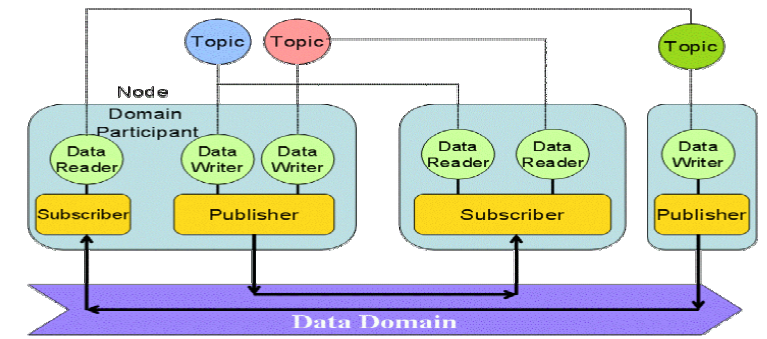
\includegraphics[width=\textwidth]{DDS_entities.png}
	\captionof{figure}{DDS entities}
\end{center}

We ran the shapes demo that came with RTI connext to get an understanding of how the framework works and what some of the QoS parameters did.

\begin{center}
	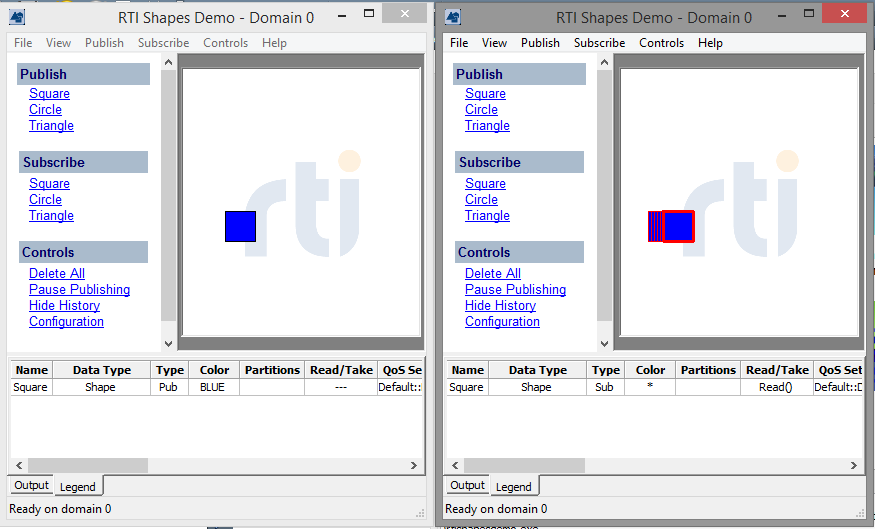
\includegraphics[width=\textwidth]{Shapes_demo.PNG}
	\captionof{figure}{RTI Connext shapes demo}
\end{center}

\subsection{Configuration on linux}

To set up RTI Connext on Linux for java development you have to set up a few different environment variables. That lets the commandline compiler find RTIs libraries. If you are using an IDE then you have to include the library from /RTI/ndds.5.0.0/class into the project.

\begin{center}
	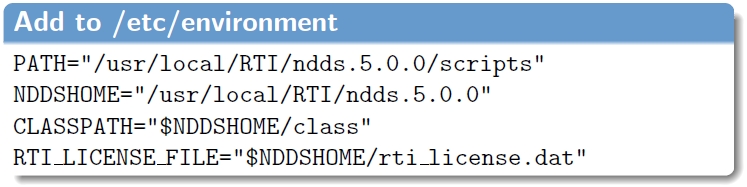
\includegraphics[width=\textwidth]{connext_environment.PNG}
%	\captionof{figure}{RTI Connext environmenvariables}
\end{center}

\begin{center}
	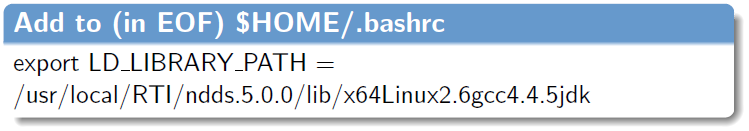
\includegraphics[width=\textwidth]{connext_environment1.PNG}
	\captionof{figure}{RTI Connext environmenvariables}
\end{center}
